\chapter{Призмы, зеркала и способы их крепления}
\section{Призмы}

\textit{Призмами} называют оптические детали или оптические системы деталей (объединенные в единый блок) с плоскими рабочими поверхностями (гранями) на которых происходит преломление или отражение оптического излучения.

В оптических приборах призмы применяют в следующих целях:
\begin{itemize}
\item для изменения хода лучей, направления оптической оси системы и направления линии визирования;
\item оборачивания изображения;
\item уменьшения габаритных размеров системы;
\item разделения или объединения пучков лучей, полей или изображений;
\item вращения  изображения  или  компенсации  поворота изображения;
\item сканирования изображения или модулирования излучения;
\item разложения света в спектр;
\item поляризации света;
\item юстировки и аттестации приборов, создания измерительных баз.
\end{itemize}

Призмы подразделяют обычно на две группы: отражательные и спектральные. К группе спектральных относят также поляризационные, модулирующие и отклоняющие излучение призмы на основе физических эффектов в их материалах при воздействии на них электрических или магнитных полей.
Самой многочисленной группой являются отражательные призмы, на примере которых рассмотрим некоторые аспекты их конструирования.По своему действию на световой пучок отражательные призмы подобны зеркалам, однако в ряде случаев призмы более эффективны, чем зеркала.

Преимущества отражательных призм по отношению к зеркалам:
\begin{itemize}
\item углы между гранями призмы неизменны, тогда как углы между зеркалами должны регулироваться с большой точностью при сборке и могут разъюстироваться в процессе эксплуатации;
\item потери света у призм от граней с полным внутренним отражением равны нулю, тогда как при отражении от поверхностей зеркал потери довольно велики; кроме того, отражающие покрытия зеркал с течением времени могут портиться;
\item конструкция крепления призм в оправах, как правило, проще, чем у системы зеркал, и обладает меньшими габаритными размерами;
\item для некоторых призм нет эквивалентных зеркальных систем (например, для призмы Дове, полупенты, некоторых видов спектральных призм).
\end{itemize}
 
Замена отражательных призм зеркалами целесообразна в случаях:
\begin{itemize}
\item когда имеют значение масса прибора, так как зеркала значительно легче призм; 
\item при высокой стоимости оптического материала;
\item для достижения требуемого качества изображения, так как призмы являются источниками хроматических и других аберраций, особенно в случаях их работы в сходящемся пучке лучей.
\end{itemize}

Рабочие и нерабочие поверхности (грани) призмы представляют собой плоскости. Рабочие поверхности подразделяют на преломляющие, через которые световой пучок входит в призму или выходит из нее, и отражательные, от которых пучок отражается при прохождении внутри призмы.

Число рабочих граней и взаимное их расположение определяют ход пучка внутри призмы и все преобразования пучка, которые при этом происходят.
Если осевой луч проходит внутри призмы в одной плоскости, то такую призму называют плоской. Если осевой луч идет в двух плоскостях, такая призма называется пространственной.

Сечение призмы плоскостью, в которой проходит осевой луч пучка, называется главным, сечением, призмы; у плоских призм одно главное сечение, у пространственных главных сечений столько, сколько плоскостей, в которых проходит осевой луч.

Отражательные призмы подразделяют на простые (их называют также одинарными), выполненные из одной заготовки материала, и составные (призменные блоки), представляющие собой комбинации из двух или большего числа простых призм, объединенных в единый блок с помощью склейки или закрепления в оправе (рис.~\ref{pic:6prism}).

\begin{figure}[h!]
	\caption{ Отражательные призмы с одним (а, в) и двумя отражениями (б) }
	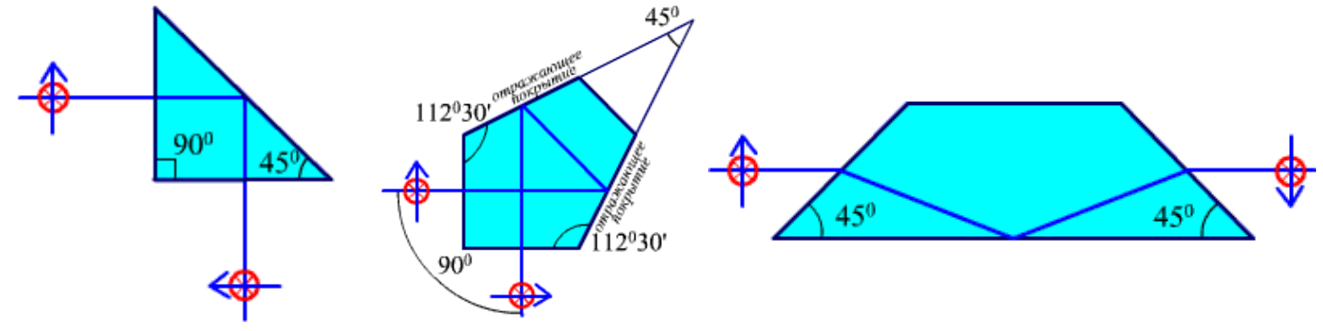
\includegraphics[width=1\textwidth]{6prism.png}
	\label{pic:6prism}
\end{figure}

Основными целевыми характеристиками отражательных призм являются: угол отклонения светового пучка, линейное смещение пучка, оборачивание изображения, степень возможности разделения или совмещения пучков лучей.

Углом отклонения называется угол между направлениями осевого луча до и после призмы, причем промежуточные отклонения луча внутри призмы во внимание не принимаются.

Линейным, смещением пучка называют расстояние между параллельными направлениями осей падающего на призму и выходящего из призмы пучка лучей. Если это расстояние равно нулю (направления осей падающего и прошедшего пучка совпадают), то такие призмы называют призмами прямого зрения (видения).

Оборачивание изображения зависит от числа отражающих граней и их расположения в пространстве.

Плоские призмы с четным числом отражающих граней дают прямое изображение. При наклоне такой призмы в главной плоскости выходящий пучок лучей не отклоняется.

Плоские призмы с нечетным числом отражающих граней дают зеркальное изображение предмета. При наклоне их в плоскости главного сечения лучи отклоняются на двойной угол.

Для оборачивания изображения в плоскости, нормальной к главному сечению, одна из отражающих граней призмы заменяется крышей, которая представляет собой две отражающие поверхности, образующие двугранный угол 90$ ^\circ $, симметрично расположенные относительно главного сечения призмы (рис.~\ref{pic:6roof}).

\begin{figure}[h!]
	\caption{ Призмы с крышей }
	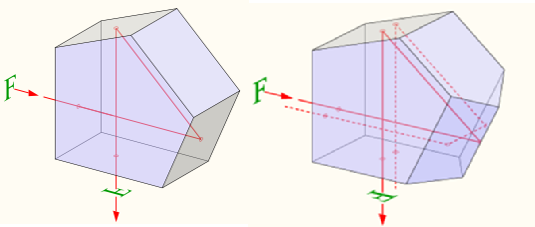
\includegraphics[width=1\textwidth]{6roof.png}
	\label{pic:6roof}
\end{figure}

Степень возможности разделения или объединения пучка лучей призмой (призменным блоком) определяется способностью разделять (объединять) пучок на две, три или более составляющих (как правило, это составные призмы типа призмы-куб, Кестерса, цветоделительной).

Типовые простые призмы, имеют условное обозначение в виде двух букв и числа, разделенных знаком тире.

Первая буква указывает число отражающих граней призмы (А -- одно отражение, Б -- два, В -- три), вторая --- характер ее конструкции (Р --  равнобедренная, П -- пентапризма\footnote{Пентапризма~-- общее название оптического устройства, служащее для поворота оси светового потока на 90$^\circ$ и удлинения его пути за счёт двух и более отражений от зеркальных поверхностей, обеспечивает минимальные внешние габаритные размеры всей сложной оптической системы}, У~-- полупента, С~-- ромбическая, Л~-- призма Лемана). Число обозначает угол отклонения осевого луча в градусах. При этом крыша считается за одну грань. Обозначается крыша индексом <<К>> у первой буквы. Для пространственных призм указываются углы отклонения в соответствующих плоскостях по ходу луча.

Типовые составные призмы, имеют другие условные обозначения. Буквой обозначают тип призмы (например, А -- Аббе-призма, К -- куб-призма, Б -- башмачная, П -- Пехана-призма), цифрой -- угол отклонения.

Составные призмы применяются в тех случаях, когда простые призмы не могут обеспечить необходимые целевые характеристики или не могут быть установлены в сходящемся пучке лучей (так как разворачиваются в наклонную плоскопараллельную пластинку и вносят большие аберрации) либо когда требуется уменьшить габаритные размеры системы.

На рис.~\ref{pic:6sostav} и ~\ref{pic:6spatial} представлены составные и светоделительные призмы.
\begin{figure}[h!]
	\caption{ Составные призмы: а, б -- башмачные, в -- Пехана, г -- Аббе }
	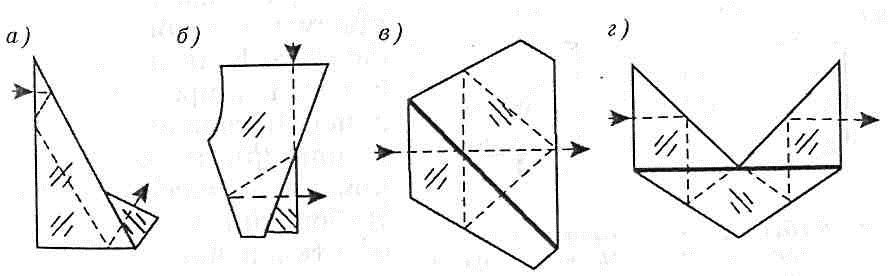
\includegraphics[width=1\textwidth]{6sostav.png}
	\label{pic:6sostav}
\end{figure}

\begin{figure}[h!]
	\caption{ Пространственные призменные системы }
	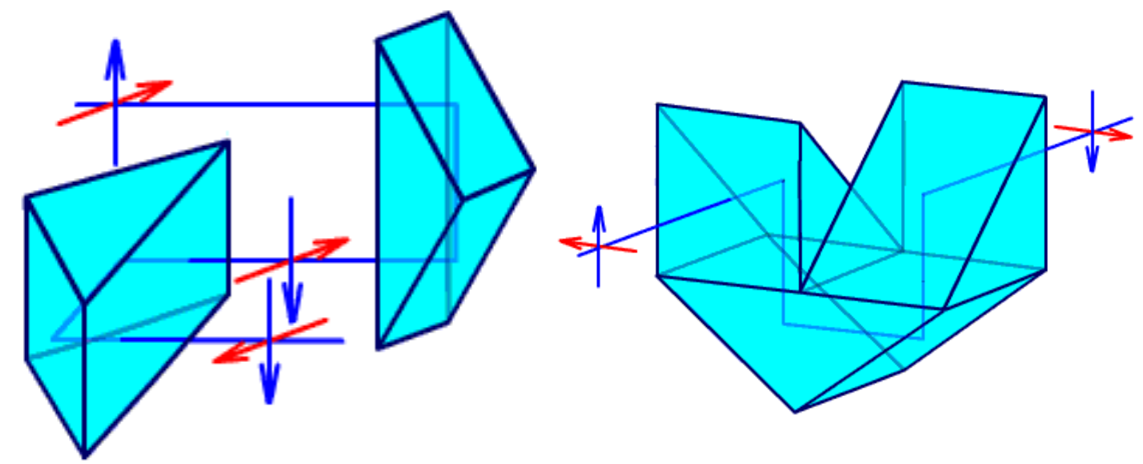
\includegraphics[width=0.7\textwidth]{6spatial.png}
	\label{pic:6spatial}
\end{figure}

На рис.~\ref{pic:6spatial} приведены составные пространственные призмы, использующиеся как оборачивающие призменные системы --- призменные системы Малафеева-Порро первого (рис.~\ref{pic:6spatial}~а) и второго рода (рис.~\ref{pic:6spatial}~б).

\textbf{Конструктивные параметры} призм, так же как и для линз, подразделяют на \textit{расчетные} и \textit{конструкторские}.

К \textit{расчетным параметрам} относят: оптические характеристики и показатели качества материала призмы, ее световые диаметры $ O_\varnothing $ на рабочих поверхностях, длину хода луча в призме $ l $, допустимые значения погрешностей изготовления рабочих оптических поверхностей (погрешности формы $ N , \Delta N$), погрешности углов призмы, влияющие на качество изображения, пирамидальность $ \pi $, вид оптических покрытий, а также (при необходимости) значения допустимой фокусности $ f_{min} $ и предел разрешения $ \varepsilon $. Эти данные определяются при габаритном, аберрационном и светотехническом расчетах оптической системы.

К \textit{конструкторским параметрам} относят габаритные размеры призмы (которые зависят от типа призмы, ее световых диаметров, запаса для крепления, юстировки), параметры фасок на ребрах и углах, допуски на углы, не влияющие на качество изображения, класс чистоты рабочих полированных поверхностей, шероховатость рабочих и нерабочих поверхностей, покрытия матовых поверхностей. Эти параметры получают в процессе разработки ее окончательной конструкции.

\section[Узлы крепления одиночных призм и призменных систем]{Узлы крепления одиночных призм и\\ призменных систем}

Призмы и призменные системы, применяемые в оптических приборах, характеризуются многообразием форм и размеров. В связи с этим существует большое количество разнообразных конструкций узлов крепления одиночных призм и составных блоков призм, достаточно полно рассмотреть которые в объеме курса лекций не представляется возможным. Рассмотрим некоторые из них.

Типовые способы крепления одиночных призм обычно классифицируют по виду основной детали, осуществляющей прижим (замыкание) призмы к рабочей поверхности оправы. Поэтому различают крепление призм накладкой, прижимными планками (лапками), угольниками, установочными винтами, пружинами, специальными деталями. Для крепления призм также используют клеи и замазки.

При разработке узла крепления любой призмы необходимо соблюдать следующие рекомендации:
\begin{enumerate}[leftmargin=*]
\item Для обеспечения точности положения призмы и исключения деформаций изгиба рабочая плоскость (плоскости) оправы должна быть чисто обработана ($ R_a $=1,25 $ \div $ 3,2 мкм) и иметь высокую степень плоскостности. При относительно больших размерах призмы на рабочей поверхности делают выборку (для выполнения принципа геометрической определенности соединения), и тогда призма базируется на два выступа по краям, либо применяют базирование на три опорные площадки.
\item Чтобы не нарушать требуемые условия преломления и отражения на рабочих гранях призмы, рекомендуется базировать призму на нерабочую грань. При базировке призмы на рабочую грань (грани) сопряжение ее с оправой должно происходить за пределами светового диаметра. При необходимости использовать для крепления или ориентации призмы грани, работающие с полным внутренним отражением, необходимо минимизировать площадь контакта между гранью и деталью крепления, например, реализовать контакт между указанными элементами по линии или точечный контакт.
\item Не допускается контакт крепежных элементов с ребрами призмы во избежание выколок стекла.
\item Между призмой и крепежным элементом (за исключением пружины) следует ставить эластичную прокладку из пробки, картона, паронита, текстолита, противоосыпочной резины или силиконового герметика, которая компенсирует погрешности размеров деталей, равномерно распределяет усилие прижима на большую площадь, предотвращает появление температурных деформаций и смещений.
\item Сопряжение призмы с рабочей поверхностью оправы отнимает три степени свободы. Базирование призмы двумя рабочими плоскостями на две плоскости оправы отнимает пять степеней свободы. Оставшиеся степени свободы призмы отнимаются соответствующим количеством ориентирующих планок.
\item Для юстировки призм следует предусматривать в конструкции их узлов возможность выполнения необходимых юстировочных подвижек.
\item Крепление склеенных призменных блоков осуществляется за одну из них, а именно -- базовую, в качестве которой выбирается наиболее массивная призма. Приклеиваемые к ней другие призмы должны иметь меньшую массу и по возможности не касаться элементов оправы.
\end{enumerate}

\begin{flushleft}
	\textbf{Крепление накладкой}
\end{flushleft}

Применяется для любых призм, имеющих параллельное расположение нерабочих граней (прямоугольная призма, пентапризма, призма Шмидта). Например, прямоугольная призма установлена нерабочей гранью на плоскость оправы (рис.~\ref{pic:6nakladka}). К оправе 1 призма прижимается накладкой~3 через эластичную прокладку 2. Накладка крепится винтами к двум стойкам, жестко соединенным с оправой. Ориентация призмы вдоль плоскости оправы выполняется при помощи трех ограничительных (ориентирующих) планок~4.

\begin{figure}[h!]
	\caption{ Крепление прямоугольной призмы накладкой }
	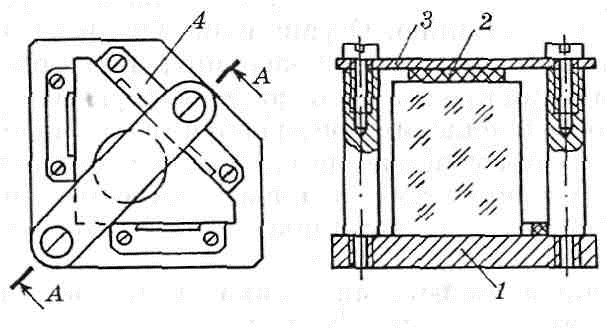
\includegraphics[width=0.8\textwidth]{6nakladka.png}
	\label{pic:6nakladka}
\end{figure}

Крепление накладкой характеризуется универсальностью, относительной простотой оправы и простотой сборки, надежностью, реализуется принцип полного внутреннего отражения на отражающих гранях, возможна юстировка призмы в оправе.

\begin{flushleft}
	\textbf{Крепление угольниками}
\end{flushleft}

Этот способ основан на использовании в узле крепления нескольких угольников различной формы (Г-образных, Z-образных). Дополнительно к угольникам применяют ориентирующие планки. Типовые конструкции крепления данным способом показаны на рис.~\ref{pic:6ugol}.

\begin{figure}[h!]
	\caption{ Крепление призм угольниками }
	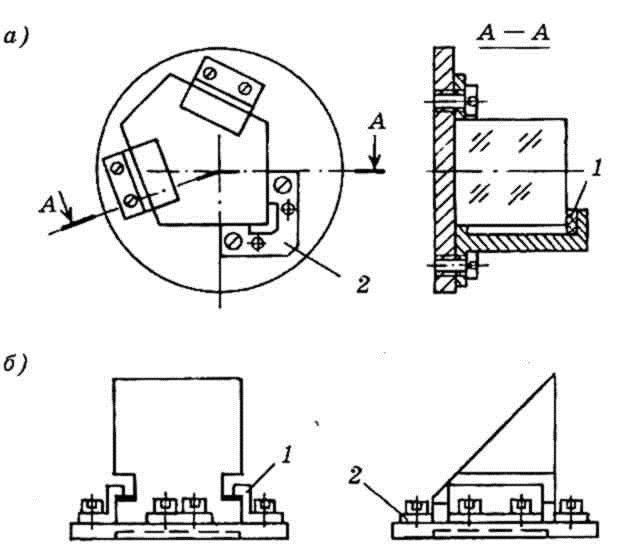
\includegraphics[width=0.8\textwidth]{6ugol.png}
	\label{pic:6ugol}
\end{figure}

Пентапризма (рис.~\ref{pic:6ugol}~а) прижимается к плоскости оправы двумя угольниками 1. Усилие прижима призмы создается в результате деформации эластичных прокладок, помещенных между призмой и угольниками. Ориентирование призмы на плоскости оправы произведено при помощи угловой планки 2, которая контактирует с преломляющими гранями призмы. После установки призмы в рабочее положение планка фиксируется штифтами.

На рис.~\ref{pic:6ugol}~б показан пример крепления угольниками прямоугольной призмы. Особенностью данной конструкции является то, что в нерабочих гранях закрепляемой призмы выполнены прямоугольные канавки. Здесь для прижима призмы к основанию оправы используются элементы канавок, через которые низкими угольниками 1 призма прижимается к основанию. Ограничение бокового перемещения призмы обеспечивается ориентирующими планками 2. Планки винтами крепятся к основанию оправы.

Этот способ крепления призм получил довольно широкое практическое применение благодаря простоте и надежности. Недостатками являются усложнение технологии изготовления снабженных канавками призм и возможность их скола при креплении.

Крепление прижимными планками. Данный способ крепления применяется для крепления сложных призм (призм с крышей, склеенных блоков), когда необходимо применить нетрадиционное базирование призмы, например -- прямоугольная призма устанавливается на гипотенузную грань.

Характерным для этого способа крепления является более сложная конструкция оправы или прижимных планок. Как правило, оправа охватывает призму с трех сторон. При этом одна (или две) поверхности базирующие, а на других - закрепляются прижимные планки. Прижимные планки бывают различными по конструкции: в виде лапок, угольников, пластин, согнутых пластин и т. п. На рис. 7 а показано крепление прямоугольной призмы с крышей. Призма установлена на катетную грань между стенками оправы с гарантированным зазором, который при необходимости выбирается эластичной прокладкой. Две пары прижимных планок ограничивают перемещение призмы в продольном и вертикальном направлениях.

На рис.~\ref{pic:6planka}~б показано крепление прямоугольной призмы, установленной гипотенузной гранью на базирующую поверхность оправы. Четыре прижимные планки привинчены к вертикальным стенкам оправы. Контакт планок с призмой выполнен по краевым зонам ее входной и выходной поверхностей. Планки выполняют упругими, либо между ними и призмой устанавливают эластичные прокладки.

\begin{figure}[h!]
	\caption{ Крепление призм прижимными планками }
	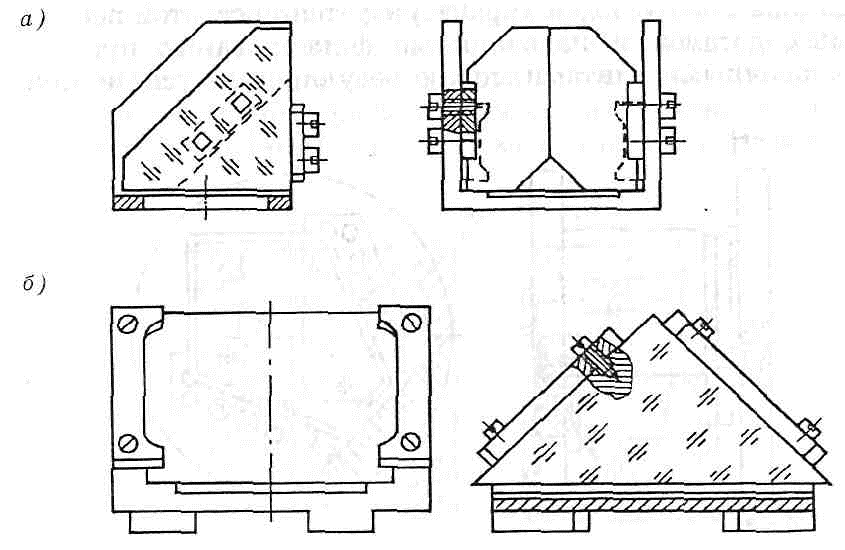
\includegraphics[width=1\textwidth]{6planka.png}
	\label{pic:6planka}
\end{figure}

Недостатком этого способа крепления является неуниверсальность и сложность деталей узла. В частности, требуется изготавливать сложные формы оправ и оригинальные прижимающие планки для каждого типа призм. Базирование на рабочие поверхности может нарушить требуемые условия отражения и вызвать воздействие недопустимых усилий. Юстировка призмы практически невозможна.

Крепление установочными винтами. Этот способ крепления рекомендуется применять для закрепления относительно больших призм с размером грани, превышающим 30 мм, когда требуется распределить усилие прижима равномерно по всей грани.

В варианте крепления пентапризмы, показанном на рис.~\ref{pic:6screw}, замыкание призмы на основание осуществляется тремя установочными винтами. Между призмой и винтами помещены эластичная и металлическая прокладки. Размеры пластин соответствуют размерам грани призмы. Металлическая пластина позволяет равномерно распределить усилие прижима по всей грани, а также предотвращает возникновение повреждений призмы при сборке. 

В свою очередь, эластичная прокладка компенсирует погрешности формы металлической пластины и изменение размеров деталей при изменении температуры. Смещения и повороты призмы вдоль основания оправы ограничиваются двумя ориентирующими планками, закрепленными на основании оправы.

\begin{figure}[h!]
	\caption{ Крепление пентапризмы установочными винтами }
	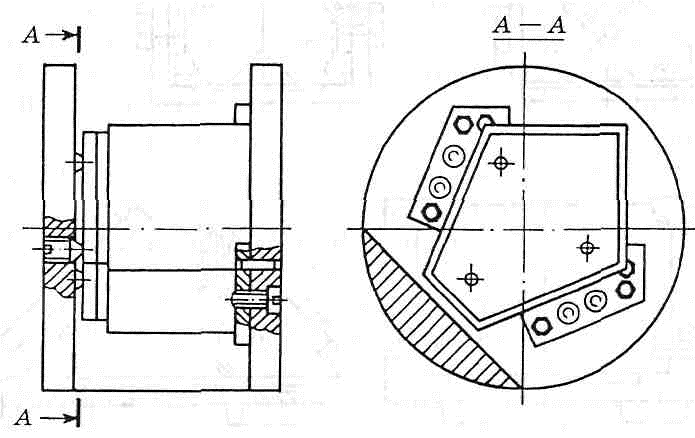
\includegraphics[width=0.9\textwidth]{6screw.png}
	\label{pic:6screw}
\end{figure}

Данная конструкция характеризуется простотой используемых деталей и надежностью фиксирования призмы. Установочными винтами можно регулировать усилие прижима. Призма защищена от внешних воздействий корпусом оправы с трех сторон.

В конструкции необходимо предусмотреть защиту от самоотвинчивания установочных винтов.

\begin{flushleft}
	\textbf{Крепление пружинами}
\end{flushleft}

Пружина как элемент крепления широко используется для закрепления призм, имеющих относительно много рабочих граней (например, прямоугольная призма с крышей). Это позволяет упростить конструкцию узла крепления. Вместе с этим пружины целесообразно использовать для прижима призмы при ее установке непосредственно в корпусную деталь прибора. В узлах крепления призм применяют пружины различных форм: тарельчатые, плоские, изогнутые, которые обычно изготавливают из пружинной стали 30X13, 65Г, У8А.

На рис.~\ref{pic:6spring} изображено крепление пружиной прямоугольной призмы с крышей. К специальной фаске на ребре призмы (90$ ^\circ $) приклеивается цилиндрический шарнир. Шарнир установлен в паз, который выполнен в корпусной детали. Вместе они образуют направляющую вращения, относительно которой можно выполнять регулировочные наклоны призмы.

Силовое замыкание призмы осуществляется изогнутой пластинчатой пружиной с закругленными краями, которые опираются на грани крыши. Регулировка усилия пружины выполняется двумя установочными винтами. При этом сила давления на призму, работающую при ударных нагрузках должна быть в 15-20 раз больше массы призмы, при работе в лабораторных приборах~-- от двух до пяти раз. Для ограничения перемещения призмы в плоскости, перпендикулярной к главному сечению (вид А-А), между призмой и крышкой корпуса установлена пластина с эластичной прокладкой.

\begin{figure}[h!]
	\caption{ Крепление прямоугольной призмы с крышей пружиной }
	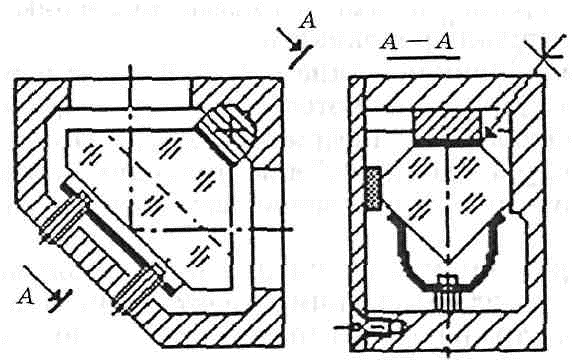
\includegraphics[width=0.7\textwidth]{6spring.png}
	\label{pic:6spring}
\end{figure}

Данная конструкция крепления позволяет выполнять угловые юстировочные подвижки призмы. Для этого при помощи двух установочных винтов изменяют усилие прижима пружины к призме. Наличие пружины обеспечивает устойчивость крепления к воздействию вибраций, толчков, а также компенсирует воздействие на узел крепления изменений температуры.

К недостаткам следует отнести необходимость физического контакта пружины с рабочими отражающими гранями призмы, который может привести не только к повреждению призмы при сборке и юстировке, но и к исчезновению эффекта полного внутреннего отражения. Поэтому площадь контакта должна быть минимальной, по возможности вне зоны светового пучка.

На рис.~\ref{pic:6planspring} показан фрагмент крепления призмы плоской пружиной. Здесь призма установлена нерабочей гранью на плоское основание оправы. Боковое перемещение призмы ограничено установочными планками. Выставленное положение призмы фиксируется пластинчатой пружиной, которая осуществляет давление на перемещающийся во втулке стержень. Для равномерного распределения усилия прижима между стержнем и гранью призмы помещены металлическая и эластичная прокладки.

\begin{figure}[h!]
	\caption{ Крепление призмы, плоской пружиной }
	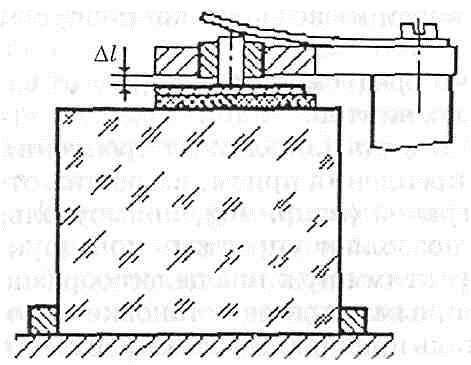
\includegraphics[width=0.6\textwidth]{6planspring.png}
	\label{pic:6planspring}
\end{figure} 

\begin{flushleft}
	\textbf{Крепление приклеиванием}
\end{flushleft}

Одной из конструктивных особенностей призм является сложность формы, отличающая их от круглых оптических деталей. Поэтому крепление призм приклеиванием, особенно имеющих небольшую массу, экономически существенно выгоднее других способов крепления.

Рассмотрим пример крепления прямоугольной призмы, у которой для использования эффекта полного внутреннего отражения, отражающая гипотенузная грань должна быть полностью свободна. Это требование наиболее просто можно обеспечить приклеиванием призмы к оправе по ее нерабочей грани (рис.~\ref{pic:6glue}). Здесь призма приклеена к боковой поверхности оправы в виде угольника, который может юстироваться с помощью винтов. Приклеивание осуществляется либо по всей поверхности сопряжения, либо по его периметру, либо по его части, например по цилиндрическому пятну 1 выборки в оправе, куда заливается герметик или другое клеящее вещество.

\begin{figure}[h!]
	\caption{ Призма, приклеенная к оправе одной гранью }
	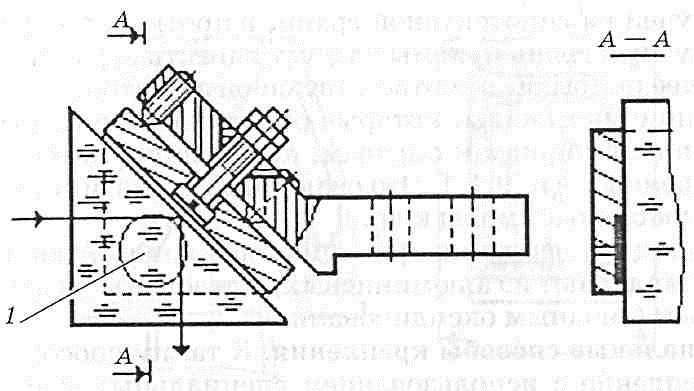
\includegraphics[width=0.8\textwidth]{6glue.png}
	\label{pic:6glue}
\end{figure} 

Недостатком такого крепления является ограничение массы приклеиваемой призмы. Клеящий слой не позволяет обеспечить надежное скрепление массивной призмы и оправы, особенно при консольном положении призмы.

Конструкция оправы (рис.~\ref{pic:6gluescrew}) позволяет осуществить надежное крепление массивной прямоугольной призмы приклеиванием. В данной конструкции высокие требования к положению призмы 1 обеспечиваются подготовкой базирующих поверхностей оправы 4. Призма установлена на краевые зоны преломляющих граней и прижимается к базовым плоскостям оправы упорным винтом 4 через пластину 2. Зазоры между оправой и призмой заполняются клеящим веществом 5. После затвердевания клея винт 4 можно удалить, а образовавшуюся пустоту заполнить клеем. Для исключения потери эффекта полного внутреннего отражения пластина 2 должна иметь выборку, соответствующую световому размеру пучка лучей на гипотенузной грани, в противном случае на гипотенузную грань призмы следует нанести зеркальное отражающее покрытие с соответствующей защитой.

\begin{figure}[h!]
	\caption{ Крепление призмы приклеиванием со вспомогательным винтом }
	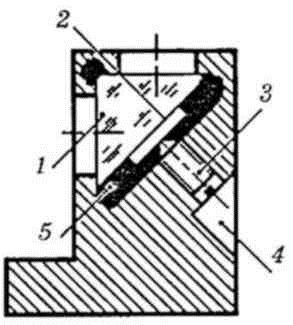
\includegraphics[width=0.35\textwidth]{6gluescrew.png}
	\label{pic:6gluescrew}
\end{figure}

Клеящие материалы, которые рекомендуется применять для крепления призм к оправам -- это различные герметики, компаунды, эпоксидные смолы.
Оправы для крепления призм приклеиванием, как правило, изготавливают из алюминиевых сплавов с последующим чернением (анодным оксидированием).
Специальные способы крепления. К таким способа относят крепление с использованием специальных крепящих деталей, либо комбинации крепящих деталей различных видов, а также крепление зажимом призм с деформированием элементов оправы, крепление формовкой призм в пластмассовые оправы, постановкой их на оптический контакт.

\begin{flushleft}
	\textbf{Конструкции узлов крепления призменных систем}
\end{flushleft}

Призмы, представляющие собой систему из двух или большего числа простых типовых призм, соединенных в единый блок с помощью склейки или закрепления в оправе, называются составными, или сложными. В склеенном блоке одна из призм, как правило, самая большая (массивная), является несущей, к ней приклеиваются остальные призмы. В узле крепления такая призма выполняет функцию базовой детали, определяющей положение других призм из склеенного блока. Крепление простых склеенных призменных блоков может быть осуществлено одним из рассмотренных выше способов крепления одиночных призм.

На рис.~\ref{pic:6shoes} приведена конструкция узла крепления башмачной призмы в оправе при помощи пружины, представляющей собой разрезанную упругую цилиндрическую трубку, которая вставляется с натягом между корпусом и прокладной пластиной, передающей силовое замыкание на призму. Базирование осуществляется по двум граням несущей призмы. Для компенсации погрешностей изготовления сопрягаемых поверхностей оправы (выполненной точным литьем) и призмы между одной из ее рабочих поверхностей и поверхностью -- оправы установлена упругая прокладка. Клин башмачной призмы установлен с необходимым воздушным промежутком (с помощью станиолевых прокладок или нанесением в вакууме дистанционных алюминиевых полосок) и приклеен к несущей призме с помощью боковых стеклянных пластин.

\begin{figure}[h!]
	\caption{ Узел крепления склеенной башмачной призмы }
	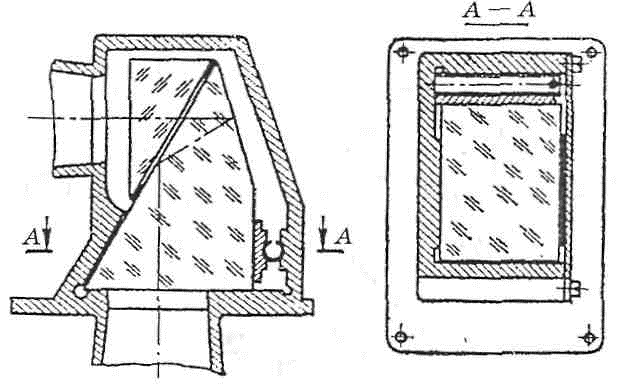
\includegraphics[width=1\textwidth]{6shoes.png}
	\label{pic:6shoes}
\end{figure}

\section{Зеркала}
\textit{Зеркалом} называют оптическую деталь, у которой рабочая поверхность (или одна из рабочих поверхностей) отражает оптическое излучение. Отражение происходит от зеркального покрытия, нанесенного на рабочую поверхность, либо от самой полированной рабочей поверхности детали, выполненной из материала, обладающего хорошей отражательной способностью (например, медные или алюминиевые сплавы, коррозионно-стойкая сталь).

Зеркальное покрытие может быть нанесено на внешнюю рабочую поверхность (наружное покрытие) или заднюю рабочую поверхность (внутреннее покрытие).
Зеркала подразделяют на плоские (с плоской рабочей поверхностью) и силовые (со сферической или асферической рабочей поверхностью).

Плоские зеркала по своему действию на световой пучок подобны отражательным призмам, а силовые~-- линзам, так как они преобразуют волновой фронт и создают изображение.

Достоинствами зеркал по сравнению с призмами и линзами являются: меньшая масса, простота конструкций, меньшее значение вносимых аберраций (в том числе отсутствие хроматизма у зеркал с наружным отражением), исключение требований к ряду показателей качества материала зеркал с наружным отражением, а также возможность создания зеркал больших размеров (до нескольких и более метров в диаметре). 

\textbf{Конструктивные параметры} зеркал подразделяют на \textit{расчетные} и \textit{конструкторские}.

К \textit{расчетным конструктивным параметрам} зеркала, получаемым в результате габаритного, аберрационного и светотехнического расчетов оптической системы, относят: световые размеры рабочей поверхности(ей) и параметры ее формы (плоскость, радиус сферы, уравнение и координаты точек для асферики), значение коэффициента отражения от рабочей (зеркальной) поверхности [при работе в УФ-области спектра (1~-- 380 нм), видимой (380~- 780 нм), инфракрасной (780~нм~-- 1 мм)]; допустимые значения погрешностей изготовления рабочей поверхности (общая и местная погрешности формы, децентрировка).

К \textit{конструкторским параметрам}, получаемым в процессе разработки конструкции зеркала, относят: материал зеркала, его габаритные размеры (зависящие от световых размеров, способа крепления, необходимой технологической и конструктивной жесткости, запаса для юстировки), шероховатость и класс чистоты поверхностей, параметры фасок, вид покрытий.

Рассмотрим некоторые особенности определения конструктивных параметров зеркал:
\begin{enumerate}[leftmargin=*]
\item Выбор материала зеркала зависит от его назначения (для построения изображения, осветительное), условий эксплуатации (температурный режим, нагрузки), требований к массе и габаритным размерам, возможности реализации необходимой технологии изготовления. 

Чаще всего зеркала изготавливают из традиционных материалов: оптического стекла (ЛК5, ЛК7, К8), плавленого кварца (КУ, KB, UVFS), ситаллов (СО115М, СО-ЗЗМ, церодур).

Развитие космической аппаратуры, создание мощных лазерных и адаптивных систем, криогенных телескопов (требующих охлаждения зеркал до температур жидкого гелия 4К и жидкого азота 77К) привели к изготовлению зеркал из нетрадиционных материалов (меди, алюминиевых сплавов, титана, бериллия, кремния, карбида кремния, боросиликата, графитоэпоксида.

Основными единичными показателями качества материала, используемого для зеркал, являются: его плотность $ \rho $ (чем она меньше, тем лучше); модуль упругости $ Е $ (чем он больше, тем лучше); температурный коэффициент линейного расширения $ \alpha $ (чем он меньше, тем лучше); теплопроводность $ \lambda $ (чем она больше, тем лучше); удельная теплоемкость $ С $ (чем она меньше, тем лучше).

Комплексными показателями качества материала являются: его удельная жесткость $ E/\rho $ , пропорциональная деформация под действием собственного веса, позволяющая оценить стабильность формы рабочей поверхности зеркала при изготовлении, закреплении и эксплуатации под действием нагрузок; температурная стабильность $ \lambda/\alpha $, характеризующая термодеформации зеркала при изменении температуры; коэффициент Максутова$ \psi = E\,\lambda/(\alpha\,\rho\,C) $, которым пользуются для ориентировочной интегральной оценки качества материала для зеркал.

Заметим, что конструктор обычно старается использовать для изготовления зеркал материалы с низким значением коэффициента $ \alpha $, однако низкая теплопроводность (температуропроводность $ q $) материала зеркала не позволяет выровнять температуру в его объеме при изменении теплового потока, что вызывает неравномерность напряжений и температурные деформации рабочей поверхности (эффект края). На это обстоятельство указывал Д.~Д.~Максутов, приводивший ряд преимуществ металлических зеркал перед стеклянными.

Металлы и другие теплопроводные материалы позволяют реализовывать альтернативный подход к решению проблемы температурной стабильности зеркал за счет их высокой теплопроводности.

Решающим аргументом в пользу ряда нетрадиционных материалов является принципиально более высокая удельная жесткость последних. Бериллий, карбид кремния, кремний превосходят традиционные материалы по этому показателю в 2-5 раз.

Особенно следует отметить карбид кремния, который сочетает удельную жесткость бериллия с температурной стабильностью лучших сверхмалорасширяющихся материалов, что позволяет создавать из этого материала зеркала с качественно новыми служебными свойствами.

Ряд нетрадиционных материалов не позволяет получать непосредственно на них рабочую поверхность оптического качества из-за пористости ($ SiC $), инородных включений ($ А1 $), токсичности при обработке ($ Be $), отсутствия технологии достижения требуемого качества поверхности ($ Ti $). В этих случаях на рабочую поверхность таких материалов наносят специальные конструкционные покрытия (стеклянные, медные, никелевые, хромовые), которые затем доводятся и полируются до оптического качества. 

\item В таблице на чертеже оптической детали, в разделе <<Требования к материалу>>, для зеркал с наружным отражением указываются категории \textit{бессвильности}, \textit{пузырности} (включения) и \textit{двойного лучепреломления}.

Вскрытые при обработке пузыри и вышедшие на поверхность зеркала свили образуют местные дефекты формы поверхности, которые искажают волновой фронт пучка, отраженного от зеркала. Пузыри (и приравненные к ним включения) влияют также на класс чистоты полированной поверхности. Двойное лучепреломление характеризует остаточные напряжения в материале зеркала, при их отсутствии затруднительно обеспечить требуемые значения $ N, \Delta N $ и возникает увеличение деформаций из-за воздействия собственного веса зеркала при его закреплении. Для зеркал с внутренним отражением указывают также и другие нормируемые для используемого материала оптические показатели качества.

\item Вид зеркального (светоделительного) покрытия выбирается в зависимости от назначения, размеров и условий работы зеркал.
Основными характеристиками всех видов покрытий являются оптические свойства (коэффициент отражения $ \rho $ и коэффициент пропускания $ \tau $), химическая стойкость, механическая и термическая прочность.

Зеркальные покрытия подразделяются на металлические, диэлектрические и металлодиэлектрические.

Простейшими металлическими отражающими покрытиями, широко используемыми для изготовления зеркал, являются металлические пленки серебра, алюминия, хрома, никеля, родия, палладия.

Серебрение дает наибольший коэффициент отражения (до 0,96), но оно наименее химически стойкое из всех покрытий -- от действия атмосферы очень быстро тускнеет и теряет отражающие свойства. В современных оптических приборах серебрение применяется только для зеркал с внутренним отражением, где защита слоя покрытия легко осуществляется нанесением на серебро тонкого слоя меди (электролитическим способом) и еще слоя защитного лака. Серебрение выполняется двумя методами -- химическим (например, из раствора азотнокислого серебра) и испарением в вакууме.

Алюминирование имеет коэффициент отражения до 0,86 и выполняется методом испарения в вакууме. Химическая стойкость алюминирования значительно выше серебрения, и при работе в лабораторных условиях оно не требует защиты; при работе во влажной атмосфере необходима защита, которая осуществляется нанесением на алюминий прозрачного слоя другого вещества (сернистого цинка, одноокиси кремния и др.). Недостатком алюминирования является низкая механическая прочность покрытия, что делает его непригодным в тех случаях, когда по условиям работы зеркало подвергается механическим воздействиям.

Благодаря хорошо освоенной технологии и высокому коэффициенту отражения алюминирование является в настоящее время основным видом покрытия для зеркал с наружным отражением, не подвергающихся механическим воздействиям.

Хромирование -- наиболее стойкое и прочное из металлических покрытий, в большинстве случаев оно не требует защиты; коэффициент отражения возможен до 0,55; применяется при работе зеркал в сложном тепловом режиме (фары, рефлекторы дуговых осветителей и т.п.), а также для зеркал полевых приборов, подвергающихся атмосферным и механическим воздействиям.

Из других зеркальных металлических покрытий часто применяют покрытия родием и палладием. Они обладают высокой химической стойкостью и механической прочностью. Коэффициенты отражения: у родиевого (с подслоем никеля или хрома) до 0,78, а у покрытия палладием до 0,68. Эти покрытия обладают высокой стойкостью при работе в агрессивных средах (морской воде, растворах кислот, щелочей и т.п.), а также при воздействии относительно высоких температур (рефлекторы прожекторов, светопроекторов), характеризуются более высокой стоимостью и сложностью технологии нанесения.

Стойкие зеркальные покрытия с коэффициентом отражения, близким к единице, получают нанесением на подложку многослойных пленочных покрытий из диэлектрических материалов. Детали с такими покрытиями получили название интерференционных зеркал.

Для изготовления интерференционных зеркал используют покрытия из нечетно чередующихся слоев диэлектриков с большими и малыми показателями преломления и оптической толщиной 0,5$ \lambda $, т.е. создают покрытия, имеющие <<антипросветляющие>> свойства. В отличие от просветляющих покрытий наружный слой интерференционного покрытия должен иметь показатель преломления больший, чем показатель подложки. С увеличением числа слоев коэффициент отражения увеличивается. Так, 15-17-слойные покрытия из пленок $ SiO_2 $ и $ TiO_2 $, $ MgF $ или $ ZnS $ имеют коэффициент отражения не менее 99\% в широкой области спектра.

Покрытия зеркал холодного света отражают свет видимой части спектра и практически полностью прозрачны для ИК-лучей, что весьма важно при применении таких зеркал в осветительных системах кинопроекционной аппаратуры.

Прочные зеркальные покрытия с коэффициентом отражения $ \rho_\lambda $ = 92 $ \div $ 99 \% получают нанесением на металлические пленки одного или нескольких слоев диэлектриков (например, тугоплавких веществ $ SiO_2 $, $ TiO_2 $ или $ ZrO_2 $). Такие покрытия называют металлодиэлектрическими, они имеют высокий коэффициент отражения в широкой полосе спектра с меньшим числом слоев пленки, чем у диэлектрических многослойных покрытий.

Светоделителъные покрытия (полупрозрачные зеркала) делят световой поток на отраженный и проходящий и характеризуются отношением коэффициента отражения $ \rho_\lambda $ к коэффициенту пропускания $ \tau_\lambda $,. Это отношение может быть получено в широком диапазоне нанесением на подложку металлических пленок разной толщины или пленок из диэлектриков. Например, светоделительные покрытия с помощью алюминирования или серебрения можно получить практически с любым соотношением между коэффициентом отражения и коэффициентом пропускания $ \rho/\tau $. 

\item Толщина зеркала зависит от его световых размеров (габаритных размеров), способа крепления и главным образом от требуемой точности рабочей поверхности.

Чем точнее должна быть форма рабочей поверхности зеркала, тем оно должно быть толще. Толстые зеркала меньще деформируются при изготовлении, закреплении и эксплуатации. Например, прогиб $ f $ круглого зеркала в виде сплошного диска, установленного горизонтально и опирающегося по периметру на три точки пропорционален четвертой степени его диаметра $ D $ и обратно пропорционален второй степени его толщины $ d $:
\[ f_{max} = 1,365*10^6\gamma (1-\mu)D^4/4\,E\,d^2 = k\,D^4/d^2, \]

где $ \gamma $ -- удельный вес материала зеркала, $ \mu $ -- коэффициент Пуассона, $ E $ -- модуль упругости, $ k  $ -- коэффициент, учитывающий механические свойства материала.

Рекомендуется применять следующие соотношения между толщиной $ d $ и наибольшим размером $ l $ (для круглого -- диаметром) зеркала, выполненного из традиционного материала:

\begin{enumerate}
\item особо точное зеркало ($ N $=0,05$ \div $0,5;  $ \Delta N $=0,02$ \div $0,1, зеркала интерферометров, концевые отражатели дальномеров, резонаторы лазеров, зеркала телескопов): $ d \ge (1/5 \div 1/7)l $;
\item точное зеркало ($ N=1\div2 $;  $ \Delta N=0,1\div0,2 $, рабочие зеркала наблюдательных, визирных, измерительных приборов): $ d \ge (1/8 \div 1/10)l $.
\item неответственное зеркало ($ N=3 \div 10 $,  $ N=0,3 \div 1 $, зеркала осветительных систем, и систем, не требующих высокого качества изображения): $ d \ge (1/11 \div 1/25)l $.
\end{enumerate}

Уменьшить толщину зеркала можно, применив при его конструировании следующие приемы:

\begin{itemize}
\item создание облегченной конструкции (сотовая структура, выполнение выборок в теле зеркала (рис.~\ref{pic:6lightmirror}~а), толщина переменного сечения (рис.~\ref{pic:6lightmirror}~б), коробчатая форма (рис.~\ref{pic:6lightmirror}~в), где к зеркалу 2 с рабочей поверхностью 1 напекается пластина 3;

\begin{figure}[h!]
	\caption{ Облегченные зеркала }
	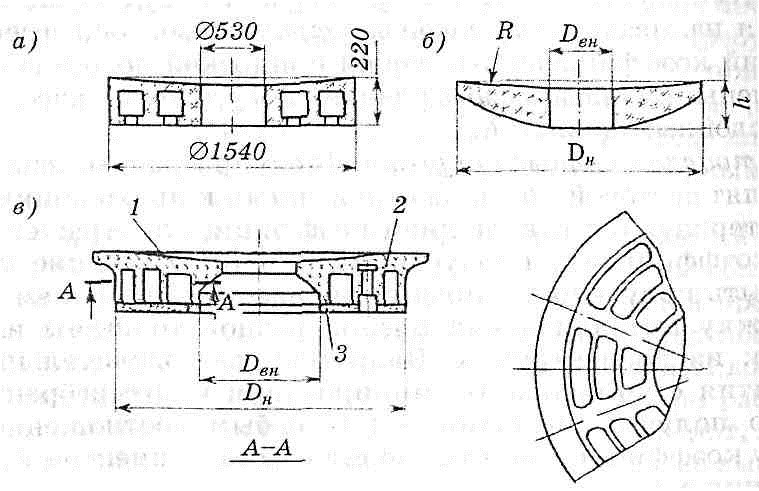
\includegraphics[width=1\textwidth]{6lightmirror.png}
	\label{pic:6lightmirror}
\end{figure}

\item разгрузка зеркала при изготовлении и креплении;
\item разработка металлостеклянной конструкции зеркала (при этом в металлической подложке выполняют выборки, уменьшающие массу конструкции зеркала).

Металлостеклянное зеркало создают путем напекания тонкой стеклянной заготовки (пластинки) толщиной в несколько миллиметров и более (при значительных размерах зеркала) на основу зеркала, выполненную из металла, сплавов, кристаллических и других материалов. Чаще всего основу таких зеркал изготавливают из металлических сплавов (титановых, коррозионно-стойкой стали, сплава ковар, алюминиевых сплавов, бериллия), для которых имеются марки стекол с близкими значениями коэффициента линейного расширения (желательно, чтобы $ \alpha $ стекла было бы меньше  $ \alpha $ материала, а их разница была бы не более $1*10^{-7} $).

После спекания стекло обрабатывается до толщины 0,2-0,3~мм и полируется до достижения рабочей поверхности требуемой точности.

Металлостеклянное зеркало обладает рядом высоких конструкционных качеств:

\begin{itemize}
\item благодаря металлической основе его можно выполнить меньшим по толщине при достаточной жесткости, а также прочности под воздействием динамических нагрузок;
\item основа зеркала может выполнять роль оправы, что снижает общую массу узла и упрощает его сборку и юстировку;
\item базовые поверхности зеркала (шейки валов под подшипники, посадочные диаметры и торцы) после полирования рабочей поверхности (как правило, до нанесения зеркального покрытия) могут быть обработаны окончательно в размер от рабочей поверхности, что может исключить необходимость его юстировки.
\end{itemize}

Заметим, что для исключения возможных деформаций стеклометаллического зеркала из-за внутренних напряжений необходимо осуществлять отжиг основы зеркала после ее механической обработки и термоциклическую обработку узла после напекания и грубого шлифования стекла.

\end{itemize}

\item Как правило, отражающий слой зеркала, используемого для построения изображения, наносят на его наружной стороне, чтобы избежать влияния отклонений характеристик материала и погрешностей изготовления преломляющей рабочей поверхности зеркала (например, погрешности формы, клиновидности) на качество изображения.

Зеркало с задней отражающей поверхностью не рекомендуется устанавливать в сходящихся пучках лучей, так как возможно возникновение двоения изображения, а при наклонном положении еще и хроматизма, астигматизма, асимметрии и других аберраций.

\item Конструктивные формы и размеры зеркал зависят от их назначения, положения в оптической системе, световых размеров (диаметра), способа их закрепления.

Наибольшее разнообразие форм имеют плоские зеркала, они бывают круглые и квадратные (если расположены нормально или под небольшим углом к пучку лучей), прямоугольные, эллиптические, многоугольные (если расположены под углом к пучку лучей).

Сферические и асферические зеркала (параболические, гиперболические, эллиптические), осевые и вне осевые обычно имеют круглую форму. Часто такие зеркала имеют внутреннее отверстие для прохождения пучка лучей, базирования зеркала или закрепления в нем других элементов (например, бленды).

Зеркала могут быть изготовлены также в виде бипризм, пирамид, конусов и полигонов (рис.~\ref{pic:6planmirror}), которые используются для разделения пучка лучей, сканирования изображения, модуляции светового потока, как эталоны углов.

Особую конструкцию имеют составные и гибкие (адаптивные) зеркала, формой рабочих поверхностей которых управляют для компенсации влияния рефракций и турбулентности атмосферы, погрешностей оптической системы и ее юстировки (рис.~\ref{pic:6adaptmirror}).

\begin{figure}[h!]
%	\caption{ Плоские зеркала: а -- одиночное зеркало, б -- зеркальный ромб, \\в -- двухсторонняя пирамида, г -- угловое зеркало, д -- четырехсторонняя пирамида, е -- светоделительное зеркало, ж -- зеркальный полигон }
	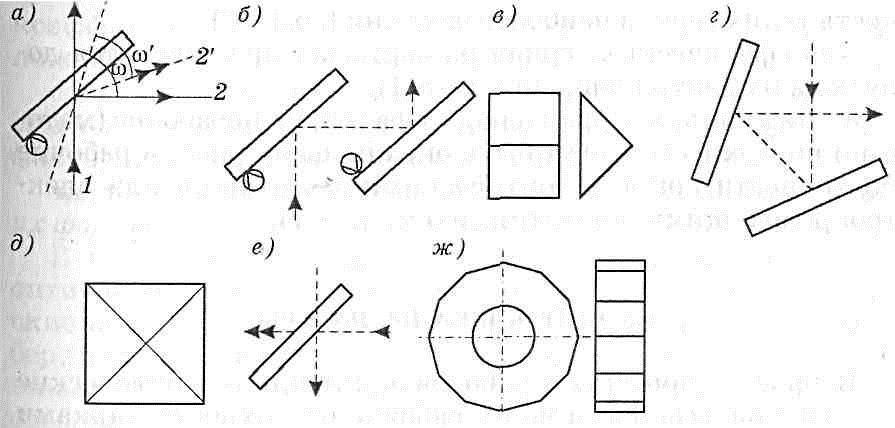
\includegraphics[width=1\textwidth]{6planmirror.png}
	\label{pic:6planmirror}
\end{figure}

\begin{figure}[h!]
%	\caption{ Адаптивное зеркало:\\ 1 -- отдельное элементарное зеркало, 2 -- цилиндр из пьезокерамики, 3 -- основание,\\ 4 -- юстировочный винт; 5 -- электрод }
	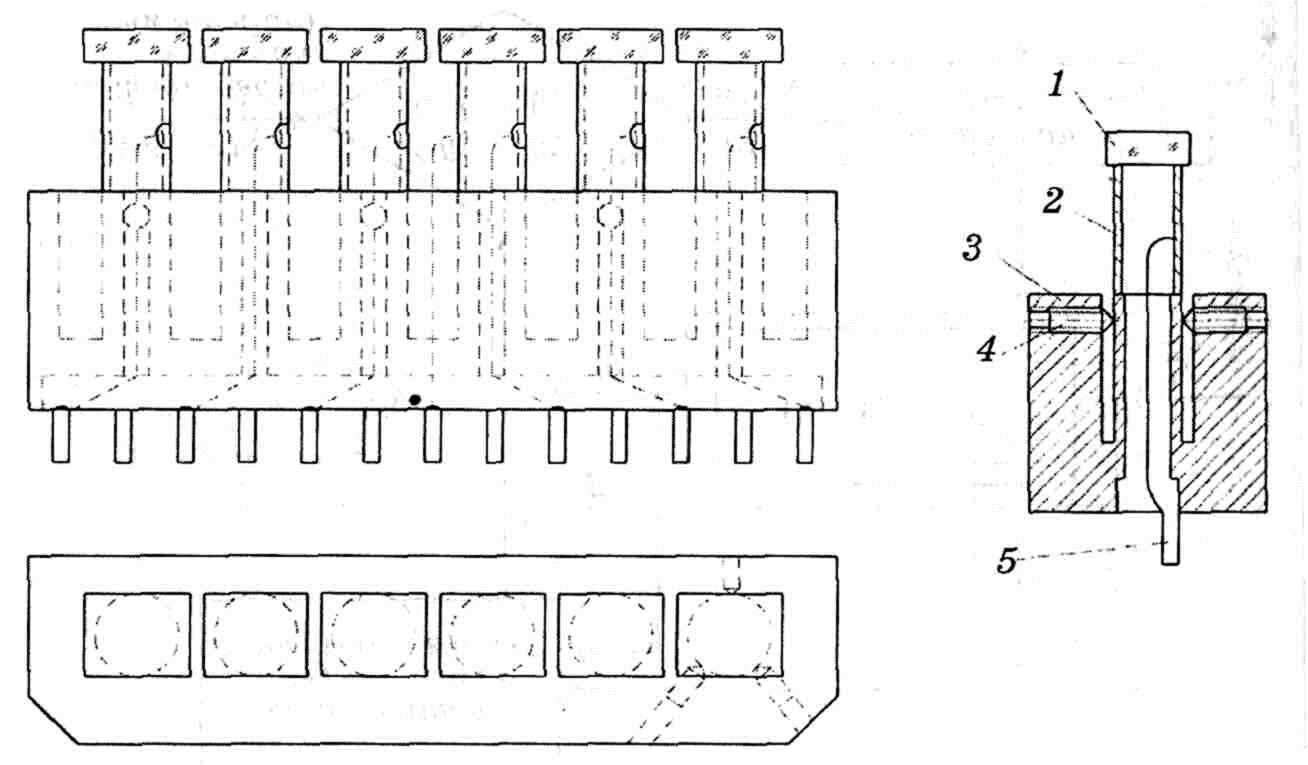
\includegraphics[width=1\textwidth]{6adaptmirror.png}
	\label{pic:6adaptmirror}
\end{figure}

\item Допуски на точность изготовления рабочих и базовых поверхностей зеркала (погрешности формы и чистоты рабочих поверхностей, погрешность посадочного диаметра (или размера) базовой поверхности, децентрировка, клиновидность рабочих поверхностей плоских зеркал с внутренним отражением) определяются  функциональным  назначением зеркала, характеристиками и требованиями к качеству оптической системы.

Например, зеркала современных телескопов и лазерных систем должны обеспечивать качество изображения и расходимость излучения на уровне предела, ограничиваемого дифракцией. Это означает, что среднеквадратичное отклонение формы оптической поверхности зеркал от заданной не должно превышать сотых долей рабочей длины волны ($ \lambda/50 \div \lambda/70 $), в линейной мере оно составляет менее 0,01 мкм. С учетом размеров зеркал (0,5~м и более) это позволяет характеризовать их как наиболее точные изделия современного приборостроения.

Допуск на погрешность формы обычно задают в виде, зависящем от метода контроля. Например, при контроле сферической поверхности с помощью интерферометра он задается в долях длины волны $ \lambda $, при контроле сферометром -- в процентах отклонения от номинального радиуса $ \Delta R $ \%, при контроле пробным стеклом -- количеством колец $ N, \Delta N $.

Заметим, что допуски на общую погрешность формы зеркал, установленных наклонно к световому пучку, более жесткие, чем для установленных перпендикулярно, а для местных погрешностей и чистоты рабочей поверхности -- наоборот, более широкие.

Для плоских зеркал с внутренним отражением их клиновидность вызывает хроматизм, а в случае светоделительных -- еще и двоение изображения. Допуск на клиновидность таких зеркал наиболее жесткий (до $ 4-6'' $).

Для сферических зеркал на чертежах проставляется допуск на их центрировку.

\item На кромках зеркал наносят фаски, их нерабочие (матовые) поверхности могут быть окрашены эмалью, а рабочие поверхности покрыты оптическими защитными или электропроводящими покрытиями.
\end{enumerate}


\section{Узлы крепления зеркал и зеркальных систем}

\begin{flushleft}
	\textbf{Требования к узлам крепления зеркал}
\end{flushleft}

Особенностью оптических зеркал, которую необходимо учитывать при разработке конструкции крепления, является их повышенная чувствительность к деформациям -- изгибу зеркала и местным искажениям формы отражающей поверхности. 

Поэтому, применяя различные способы крепления (при помощи планок, скоб, угольников, резьбовых колец, пружин и других прижимных элементов, а также клеев и замазок), необходимо соблюдать следующие условия:
\begin{enumerate}
\item Конструкция крепления зеркала должна обеспечивать статически и геометрически определенное соединение --- базирование на три точки (площадки).
\item При разработке конструкции необходимо соблюдать принцип силового замыкания соединений: сила, прижимающая зеркало, должна проходить через опорные площадки оправы. В узлах крепления больших (массивных) зеркал, кроме того, необходимо применять принцип равномерного распределения его массы путем введения в конструкцию дополнительных опор (механическая разгрузка), а также гидравлических или пневматических разгрузок.
\item Между прижимающей деталью и зеркалом рекомендуется ставить упругие прокладки, чтобы не вызывать локальных (в местах контакта) напряжений.
\item Следует обеспечивать необходимую жесткость конструкции, используя зеркала и оправы «сотовой» структуры, а также зеркала, не нуждающиеся в оправах.
\item Следует предусматривать необходимую юстировку зеркала относительно оправы, либо оправы зеркала относительно корпусных деталей и баз устройства (системы).
\end{enumerate}

К мерам, позволяющим снизить воздействия на узел крепления зеркала колебаний температуры, относятся следующие:
\begin{itemize}
\item обеспечение необходимого температурного зазора в посадке зеркала в оправу;
\item подбор материалов зеркала и оправы с близкими значениями коэффициентов линейного расширения (например, стекло «крон» и металл титан; зеркало из кварца или ситалла, а оправа из сплава инвар);
\item применение промежуточных (между зеркалом и оправой) компенсационных элементов, термокомпенсаторов;
\item консольное крепление зеркала;
\item изготовление зеркал из металла или в виде металлостеклянного зеркала, не нуждающихся в оправах и обладающих хорошей температурной стабильностью.
\end{itemize}

Круглые зеркала могут быть закреплены в оправах теми же способами, что и рассмотренные выше способы крепления круглых линз. 

Рассмотрим типовые конструкции узлов крепления некруглых и круглых зеркал.

\newpage
\begin{flushleft}
	\textbf{Крепление при помощи прижимных планок}
\end{flushleft}

Крепление при помощи прижимных планок (лапок, угольников, пластин) применяется для точных зеркал различных форм и размеров. Зеркало устанавливается на три выступающие площадки плоской оправы (рис.~\ref{pic:6plankamirror}~а). Площадки могут быть заменены прокладками из алюминиевой фольги, если размер зеркала не превышает 50~мм. Прижим зеркала осуществляется Z-образными планками, которые винтами крепятся к оправе в местах расположения выступающих площадок. Для компенсации погрешностей сопряжения <<зеркало~-- планка>> между ними помещается эластичная прокладка (картон, пробка, паронит).

Если силы трения не обеспечивают неподвижность зеркала, планки выполняют дополнительную функцию -- ограничивают перемещение зеркала вдоль оправы путем создания контакта планок по краю зеркала. Для этого на планках выполняют выступ~В.

\begin{figure}[h!]
%	\caption{ Крепление зеркала:\\ а -- Z-образными планками, б -- Г-образными планками }
	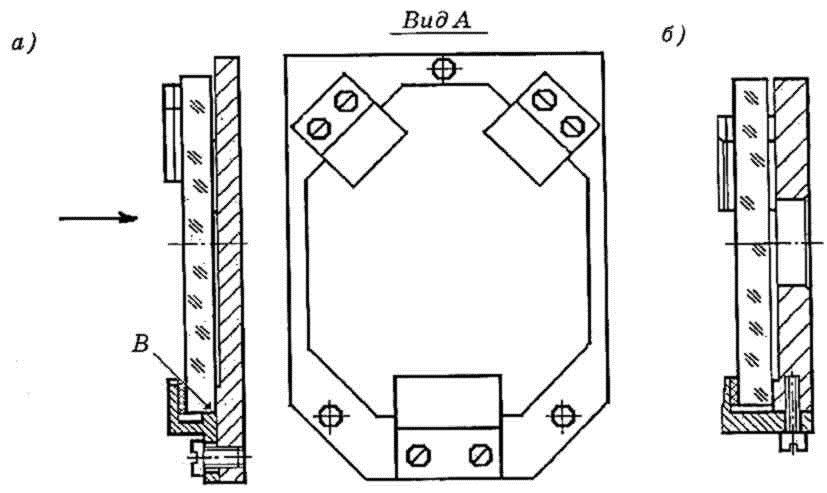
\includegraphics[width=1\textwidth]{6plankamirror.png}
	\label{pic:6plankamirror}
\end{figure}

Придание прижимным планкам Г-образной формы (рис.~\ref{pic:6plankamirror}~б) позволяет регулировать усилие прижима зеркала за счет смещения планок в пределах зазора в отверстиях под крепежные винты.

Недостатками конструкции являются: ограниченность в компенсации воздействия колебаний температуры, увеличение габаритных размеров и снижение технологичности узла крепления из-за применения нескольких крепежных элементов.

К положительным свойствам можно отнести простоту сборки узла, возможность крепить зеркала любой конфигурации. Конструкция удовлетворяет основным требованиям к узлам крепления зеркал.

\begin{flushleft}
	\textbf{Крепление при помощи пружин}
\end{flushleft}

Данный способ крепления основан на создании замыкающего усилия для прижима зеркала к оправе при помощи пружины (проволочной, мембранной, пластинчатой). На рис.\ref{pic:6springmirror} приведена конструкция крепления круглого зеркала проволочной пружиной. Здесь зеркало устанавливается на кольцевой уступ оправы по посадке с гарантированным зазором. Прижим зеркала осуществляется диском с выборкой в центре, на который воздействует винтовая пружина сжатия (в конструкции могут быть применены и другие типы пружин). Усилие прижима регулируется винтом, положение которого фиксируется гайкой. Для равномерного распределения усилия по окружности соединение диска со штоком может быть шарнирное.

\begin{figure}[h!]
	\caption{ Крепление зеркала пружиной }
	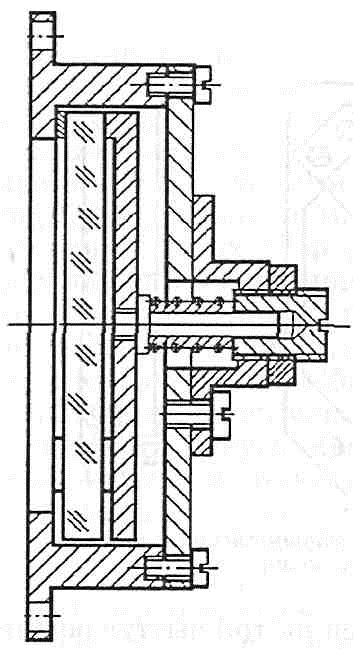
\includegraphics[width=0.3\textwidth]{6springmirror.png}
	\label{pic:6springmirror}
\end{figure}

При креплении рассмотренным способом зеркал средних и больших диаметров, чтобы исключить возможные изгибающие моменты, зеркало должно базироваться на три площадки. Поэтому между зеркалом и уступом оправы через 120$ ^\circ $ помещают металлические прокладки либо выполняют в уступе выборки, создающие на нем три опорные площадки. В прижимающей зеркало пластине должны быть выполнены выборки, чтобы образованные выступы были сориентированы напротив установленных прокладок.

Достоинством крепления пружиной является обеспечение стабильности формы и положения зеркала при механических воздействиях и воздействии колебания температуры, так как возникающие возмущения компенсируются за счет деформации пружины.

К рассмотренным механическим способам крепления, для круглых зеркал можно добавить крепление при помощи резьбового кольца или проволочным кольцом, аналогично креплению линз.

\begin{flushleft}
	\textbf{Крепление приклеиванием}
\end{flushleft}

Конструкции крепления зеркал приклеиванием отличаются в зависимости от размеров, формы и назначения зеркал в оптической системе.

Для зеркал неответственных систем (осветительных c $ N=5,\, \Delta N=0,5 $) возможно крепление по плоскости с опорой на равномерный сплошной слой клеящего вещества, например, герметика марки УТ-34. На рис.~\ref{pic:6sphermirror} показано крепление сферического зеркала 3 диаметром 48~мм из стекла К8 в оправе~2 из алюминиевого сплава. Зеркало помещено на слой герметика 1 толщиной 0,5~мм, нанесенного на плоскость оправы. Эта конструкция, из-за разделения оправы и зеркала клеящим слоем, не обеспечивает высокой точности положения зеркала относительно базовых поверхностей оправы. 

\begin{figure}[h!]
	\caption{ Крепление сферического зеркала на слой клеящего вещества }
	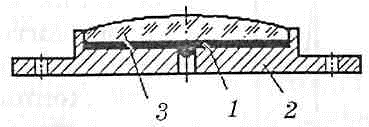
\includegraphics[width=0.4\textwidth]{6sphermirror.png}
	\label{pic:6sphermirror}
\end{figure}

\begin{figure}[h!]
	\caption{ Крепление зеркала с установкой на опорные пояски }
	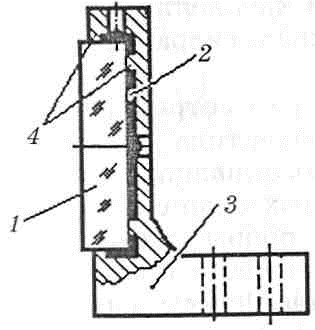
\includegraphics[width=0.35\textwidth]{6poyasok.png}
	\label{pic:6poyasok}
\end{figure}

В конструкции узла, показанного на рис.~\ref{pic:6poyasok}, устранен недостаток неопределенного базирования зеркала. Для этого зеркало~1 установлено на специально выполненные в оправе~3 опорные пояски~4 шириной 0,5~мм. Клеящее вещество~2 залито в промежутки между поясками. В оправе выполнены отверстия для выдавливания излишков клеящего вещества. Эта конструкция позволяет разделить функции: элементы оправы обеспечивают базирование (ориентацию) зеркала, клеящее вещество обеспечивает соединение (закрепление) зеркала с оправой.

Для крепления сферических зеркал (рис.~\ref{pic:6cylindric}), имеющих в центре отверстие, можно использовать его внутреннюю цилиндрическую поверхность.

\begin{figure}[h!]
	\caption{ Крепление зеркала за цилиндрическое отверстие }
	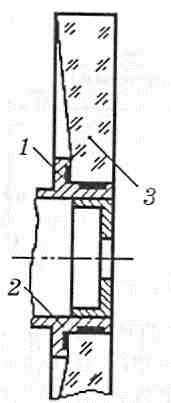
\includegraphics[width=0.2\textwidth]{6cylindric.png}
	\label{pic:6cylindric}
\end{figure}

Оправа~2 представляет собой полую ось с фланцем. Она изготовлена из алюминиевого сплава~Д16Т, имеет черное покрытие~-- анодное оксидирование. Особенностью оправы является наличие центрирующих поясков, на которые устанавливается зеркало~3. Поскольку именно эти элементы определяют относительное положение зеркала, в рабочем чертеже оправы следует установить допуск отклонения от перпендикулярности между осевыми и радиально расположенными поясками. Клеящее вещество~1 заливают в промежутки между поясками по цилиндрической и плоской части оправы. Глубина промежутков, как правило, не превышает~0,5~мм.

\begin{flushleft}
	\textbf{Специальные способы крепления}
\end{flushleft}

К ним относятся крепления крупногабаритных зеркал, металлостеклянных, консольные виды крепления, крепления свариванием, спеканием или постановкой на глубокий оптический контакт деталей (зеркал и оснований). Крепление крупногабаритных зеркал (более 200~мм) отличается от обычных, рассмотренных выше, способов крепления. Базирование таких зеркал только на три опоры хотя и является статически определенным, но приводит к недопустимым прогибам отражающей поверхности из-за статической деформации зеркала. Причем значение деформации прямо пропорционально четвертой степени диаметра зеркала. Поэтому в конструкциях крепления таких зеркал количество опор в направлении силы тяжести увеличивается. При этом важно сохранить принцип трехточечного базирования и учитывать изменяющееся положение зеркала в процессе работы. Существуют различные системы осевой и радиальной разгрузки при креплении зеркал в оправах (Гребба, Ласселя, пневматическая, гидравлическая).

Выполнение указанных требований рассмотрим на примере крепления главного зеркала объектива телескопа (рис.~\ref{pic:6razgruzka}). Зеркало установлено на восемнадцать разгрузочных опор~1. Соединение разгрузочных опор с зеркалом выполнено герметиком. Каждые три опоры объединены треугольной платформой~2. В центре тяжести платформы установлен шаровой шарнир. По две платформы через эти шарниры соединены с плечом рычага. Рычаги закреплены на общей оправе также через шаровые шарниры~3. Такая конструкция обеспечивает равномерное распределение массы зеркала относительно всей поверхности. Соединение опор с зеркалом эластичным материалом позволяет существенно упростить конструкцию разгружающей опоры и компенсировать погрешности сопрягаемых элементов, что не вызывает деформацию зеркала. Вместе с этим конструкция требует тщательной сборки и настройки, прежде всего, выравнивания усилий, создаваемых разгрузочными устройствами.

\begin{figure}[h!]
	\caption{ Разгрузка массы зеркала на 18 опор: 1 -- опоры, 2 -- разгрузочная площадка, 3 -- сферический шарнир }
	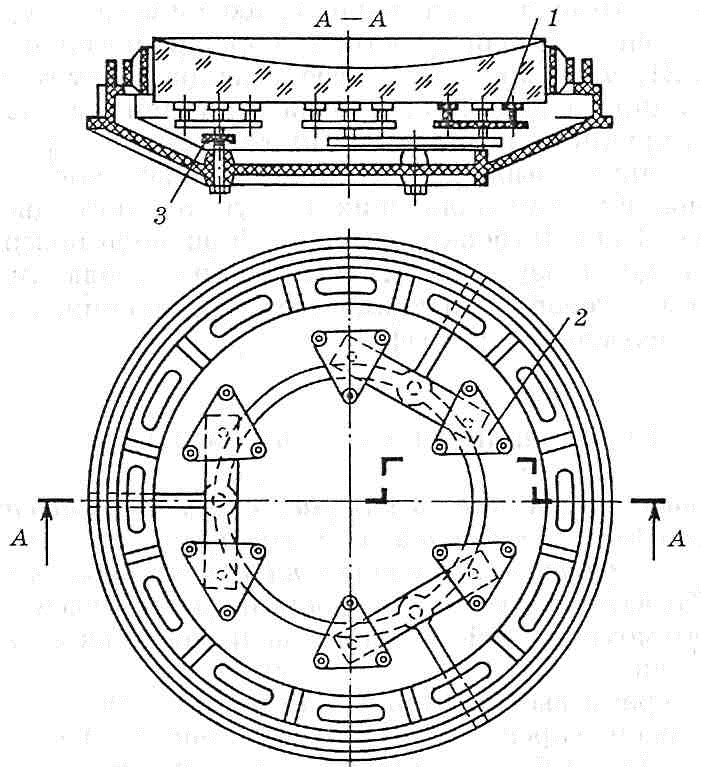
\includegraphics[width=0.85\textwidth]{6razgruzka.png}
	\label{pic:6razgruzka}
\end{figure}

На рис.~\ref{pic:6razgruzka1}~ показаны примеры конструкций для разгрузки массы зеркала. Изображения зеркал с сотовой структурой показаны на рис.~\ref{pic:6channelMirror}.

\begin{landscape}
	
	\begin{figure}[h!]
		\caption{ Пример конструкций для разгрузки массы зеркала }
		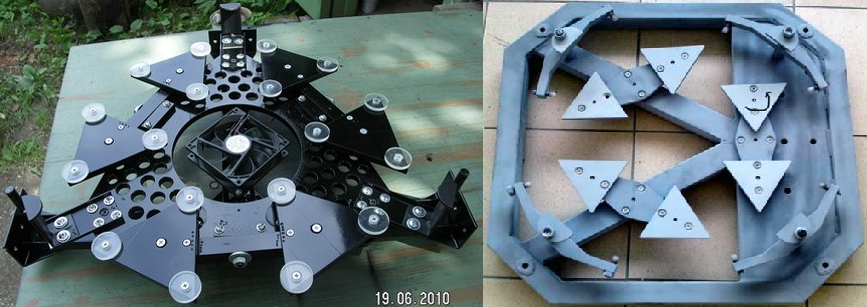
\includegraphics[width=0.75\textwidth]{6razgruzka1.png}
		\label{pic:6razgruzka1}
	\end{figure}
	
	\begin{figure}[h!]
		\caption{ Примеры зеркал с сотовой структурой }
		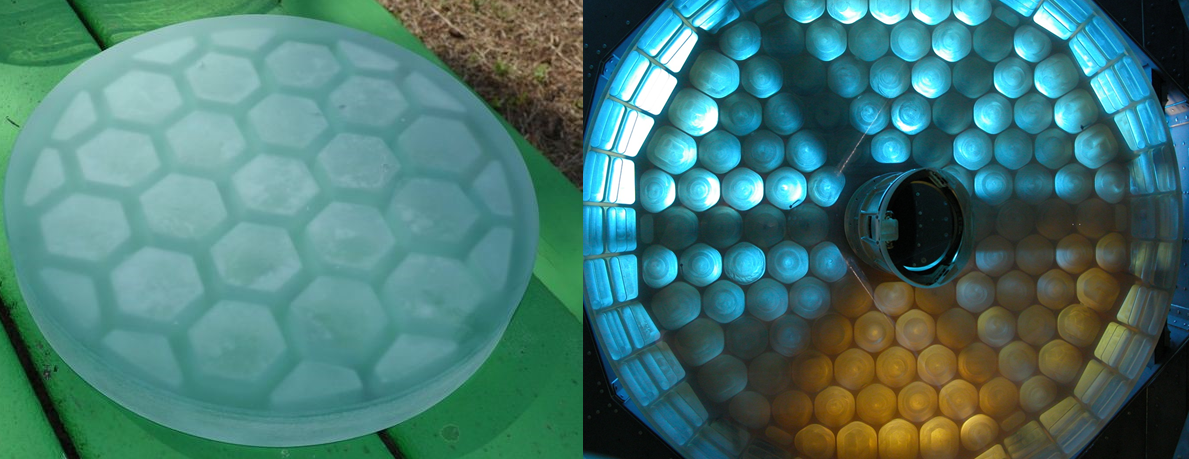
\includegraphics[width=0.75\textwidth]{6channelMirror.png}
		\label{pic:6channelMirror}
	\end{figure}
	
\end{landscape}

\begin{flushleft}
	\textbf{Крепление зеркальных систем}
\end{flushleft}

К узлам крепления зеркальных систем предъявляются те же требования, что и к узлам крепления одиночных зеркал. Кроме того, узел крепления зеркальной системы должен обеспечивать требуемое взаимное расположение рабочих (отражающих) поверхностей отдельных зеркал. В наиболее ответственных случаях предусматриваются механизмы регулировки угла между зеркалами.

На рис.~\ref{pic:6doublemirror} приведена конструкция узла крепления двухзеркальной системы с углом отклонения лучей 180$ ^\circ $. Зеркала~5 установлены на опорные поверхности корпуса~3, выполненные каждая в виде трех выступающих площадок, и прижимаются к ним при помощи винтов~8 через упругие пластины~6. Каждый из упоров~9 пластины располагается напротив опорной площадки. В основании корпуса выполнены отверстия для входа и выхода светового пучка. Винты~8 завинчены в крышки~7 с гайками~1 и фиксируются контргайками~2. Крышки привинчены к корпусу винтами~4.

\begin{figure}[h!]
	\caption{ Двухзеркальная система с углом отклонения лучей 180$ ^\circ $ }
	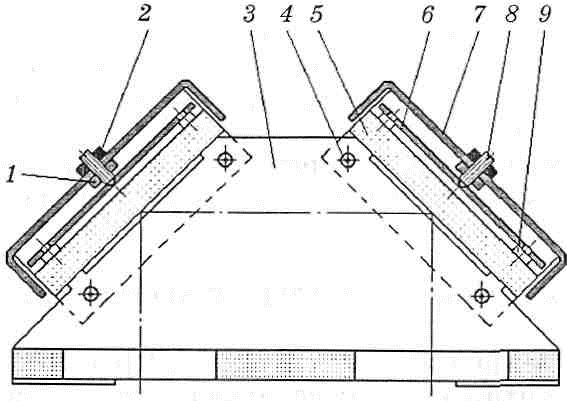
\includegraphics[width=0.7\textwidth]{6doublemirror.png}
	\label{pic:6doublemirror}
\end{figure}


